\clearpage
\setcounter{page}{1}

\section{Langkah Kerja}
\begin{enumerate}

\item Pertama buka oracle apex, jika belum memiliki akun oracle yang terbaru maka klik get started for free\\
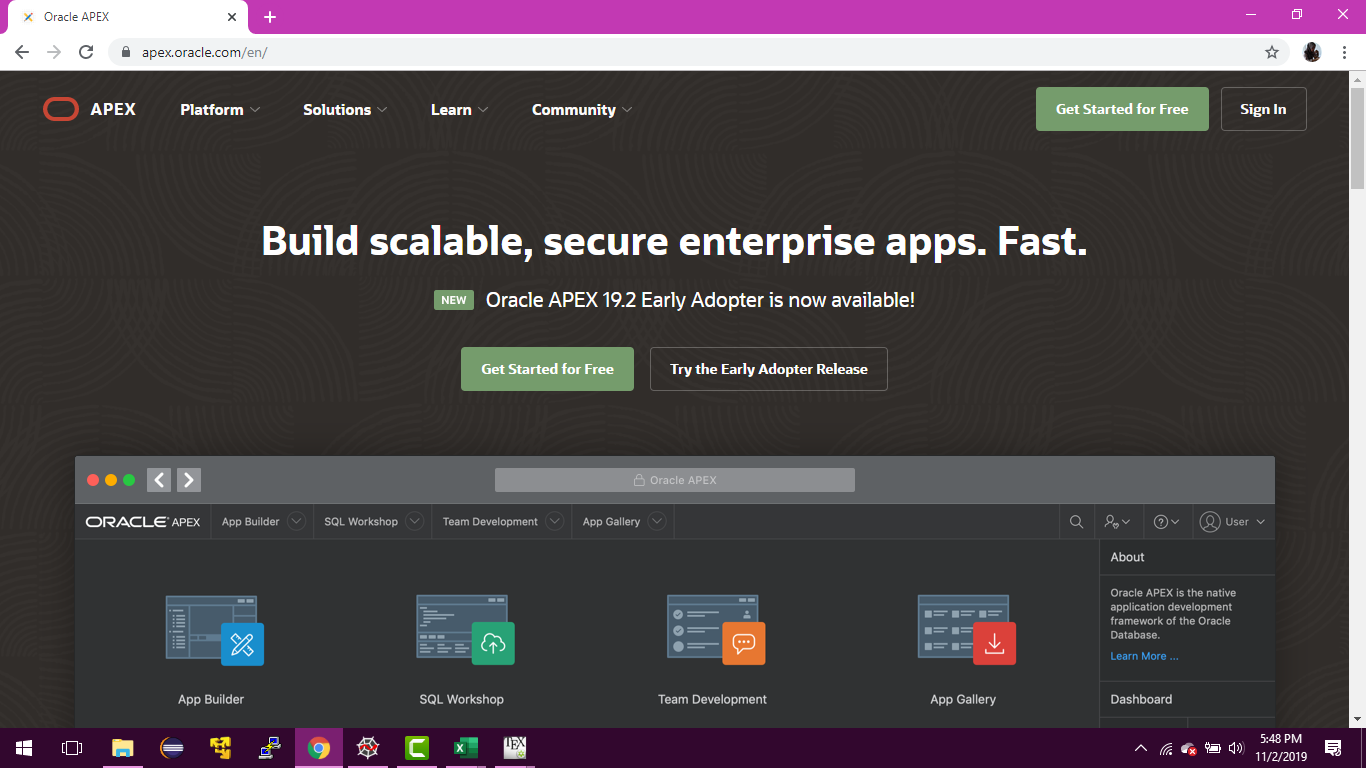
\includegraphics[scale= 0.3]{gambar/1.png}\\
\item Klik request a free workspace\\
Lalu isi sesuai dengan data sampai langkah terakhir.\\
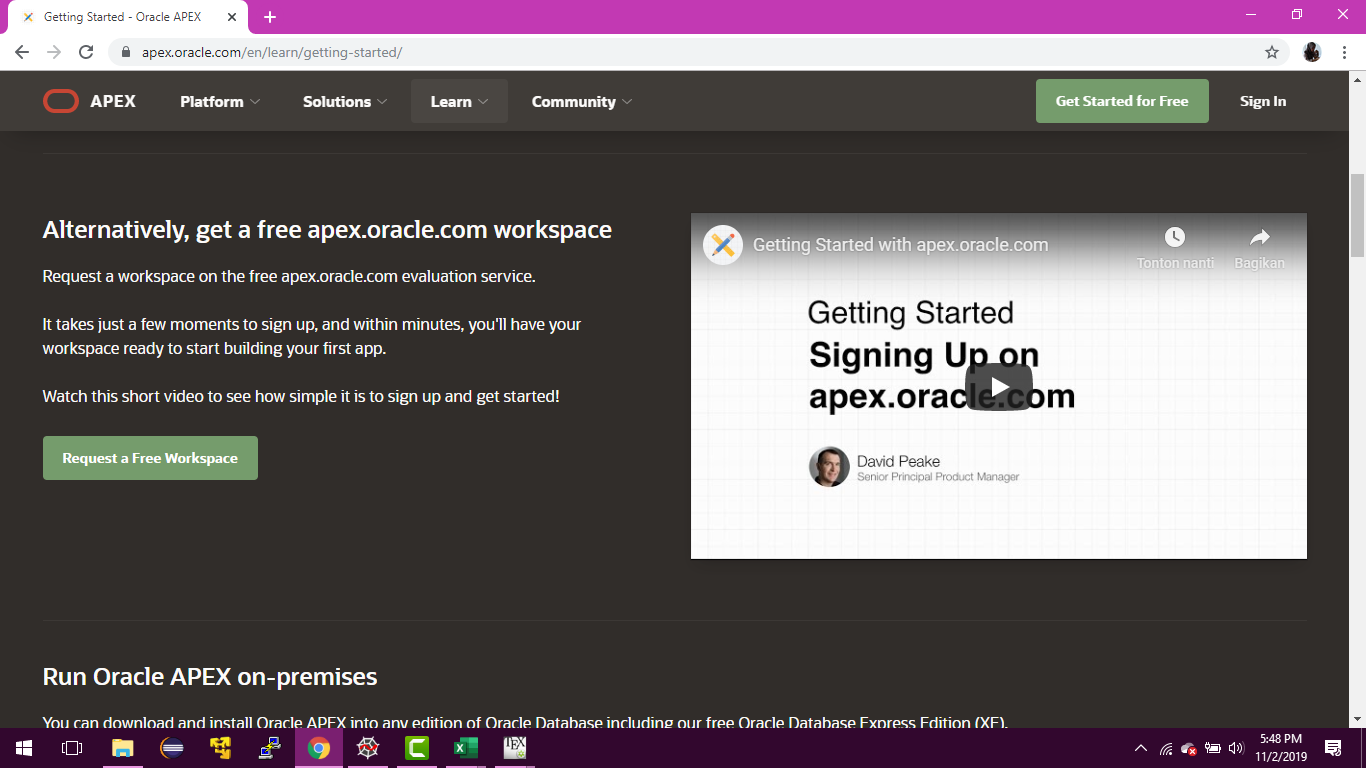
\includegraphics[scale= 0.3]{gambar/2.png}\\
\item Jika sudah memiliki account, maka klik sign in dan masukan nama workspace anda\\
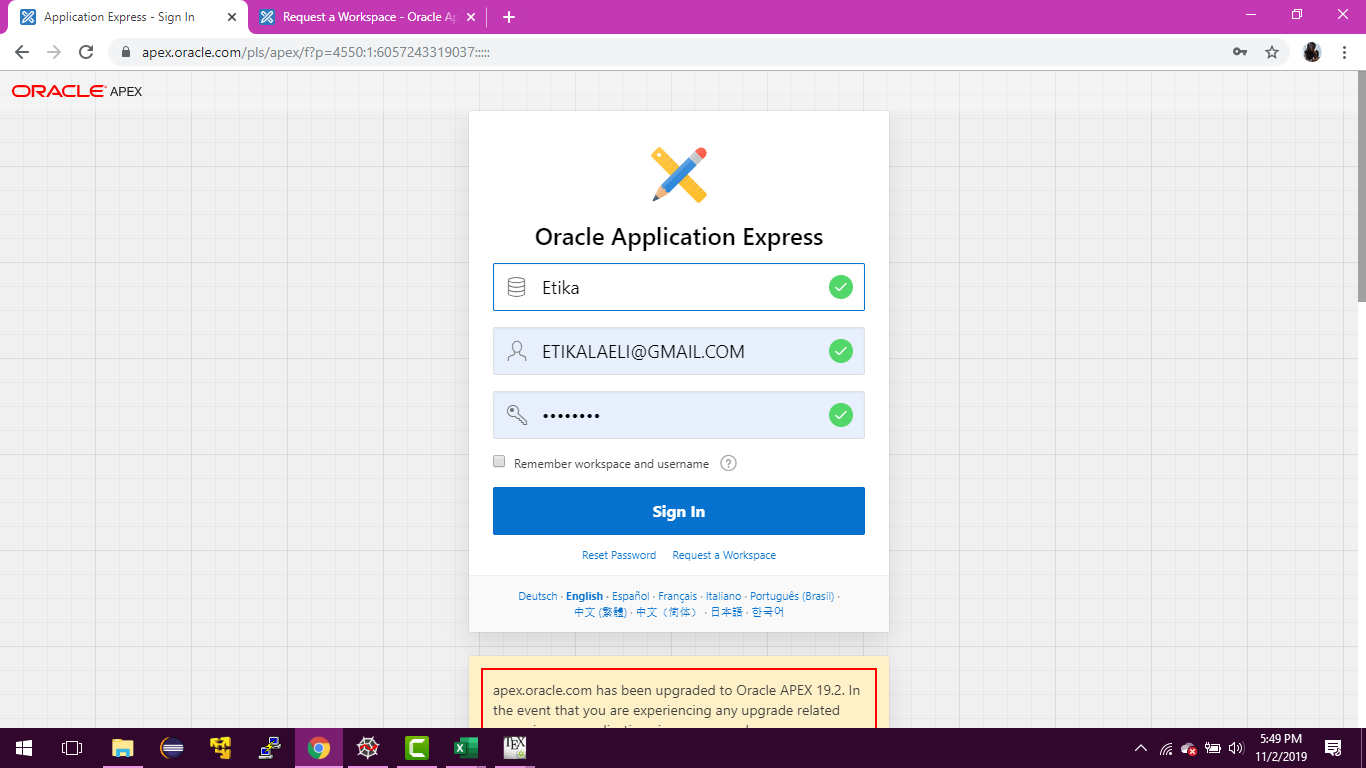
\includegraphics[scale= 0.3]{gambar/3.png}\\
\item klik App Builder untuk langkah pertama membuat aplikasi\\
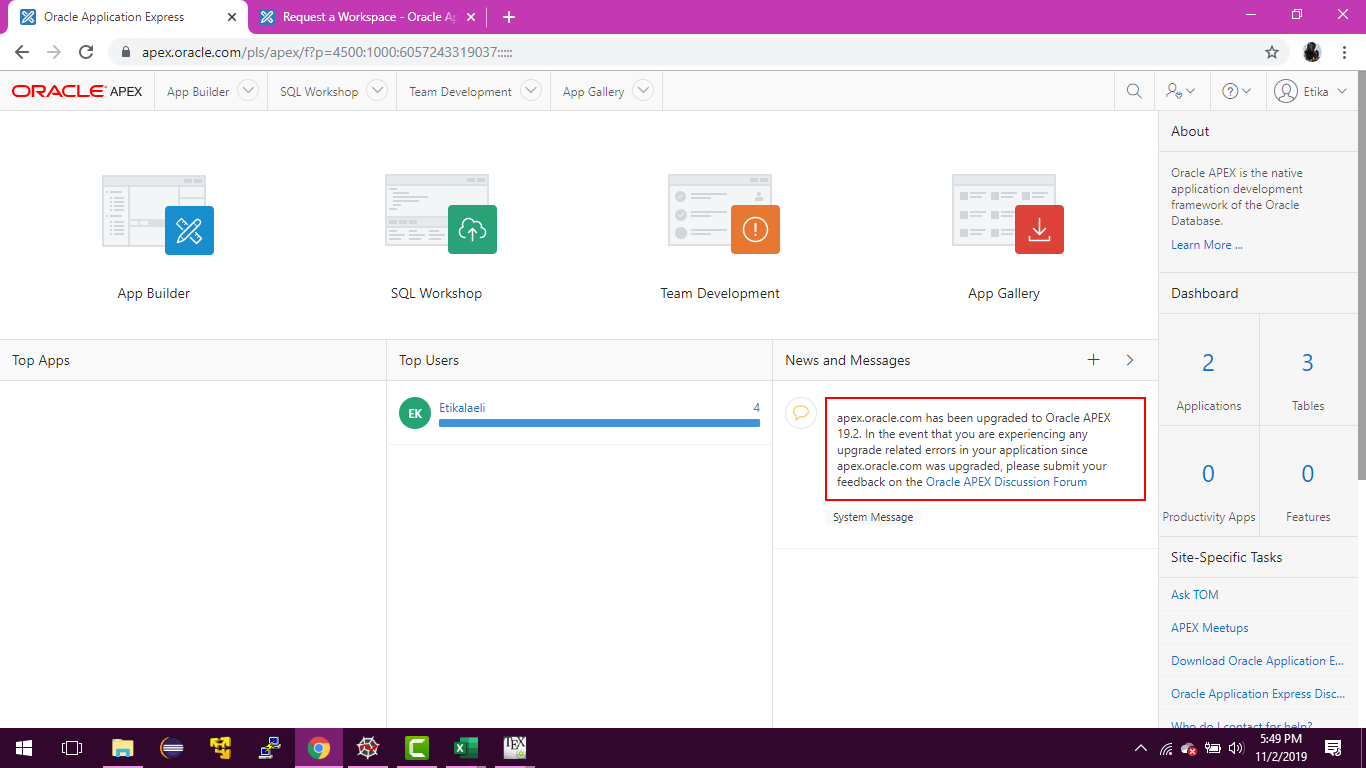
\includegraphics[scale= 0.3]{gambar/4.png}\\
\item setelah klik App Builder klik create untuk membuat aplikasi\\
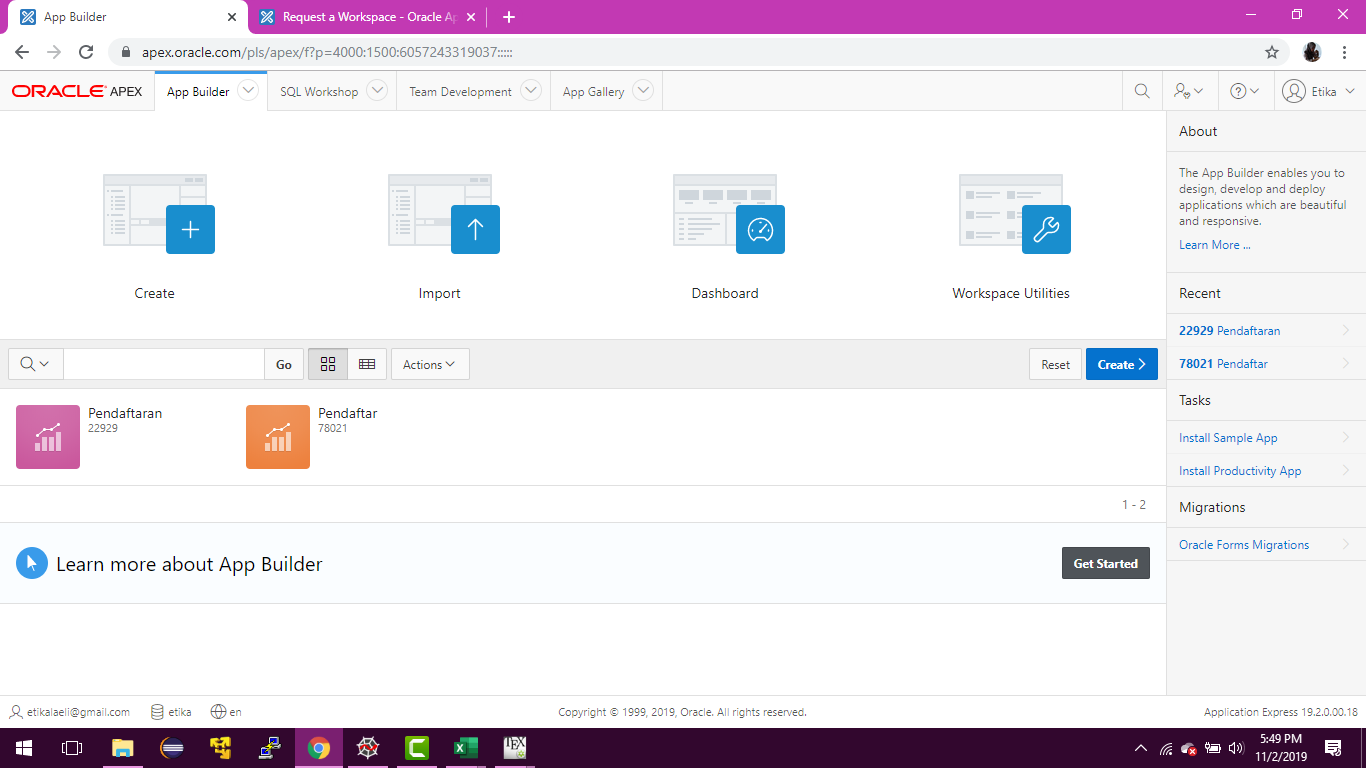
\includegraphics[scale= 0.3]{gambar/5.png}\\
\item klik from a file untuk memilih file mana yg akan dijadikan isi tabel dan pastikan tabel sudah csv.\\
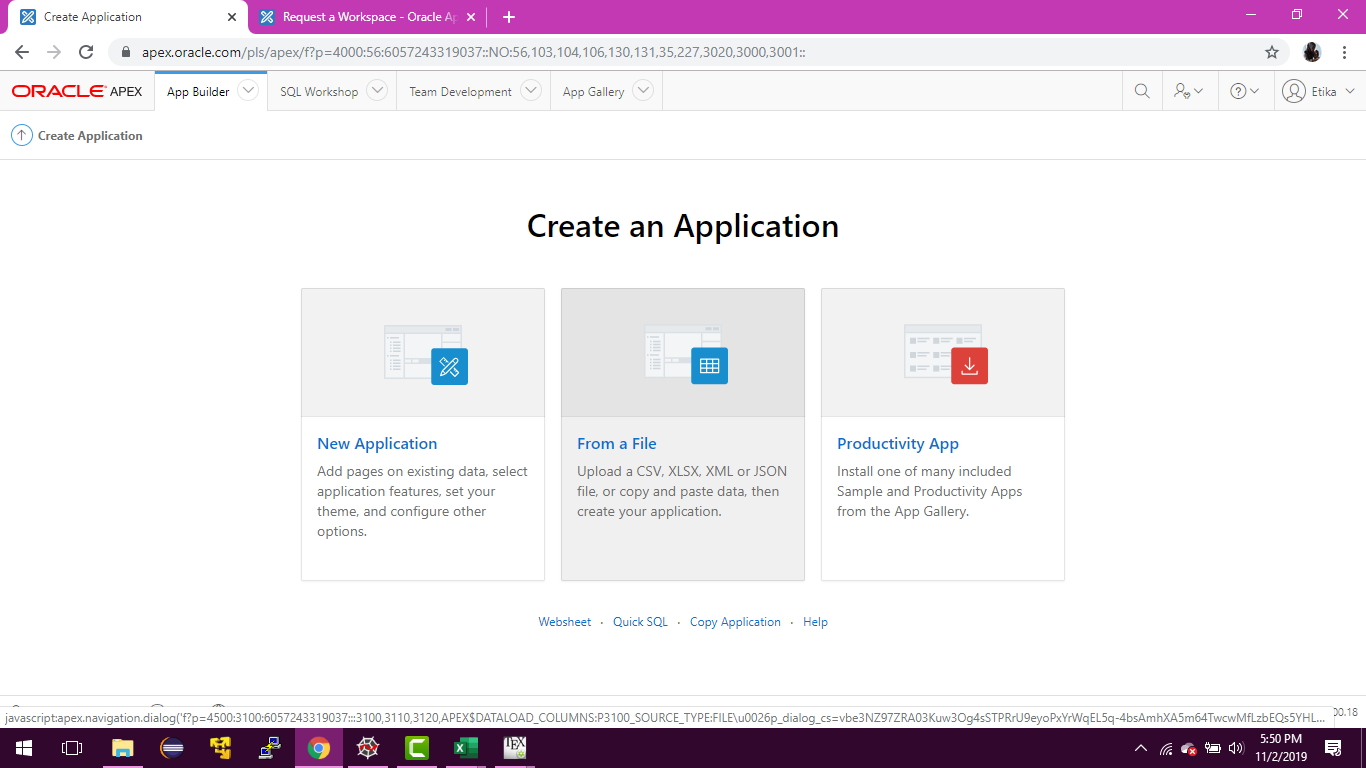
\includegraphics[scale= 0.3]{gambar/6.png}\\
\item drug dan drop file yang akan dijadikan isi dalam tabel\\
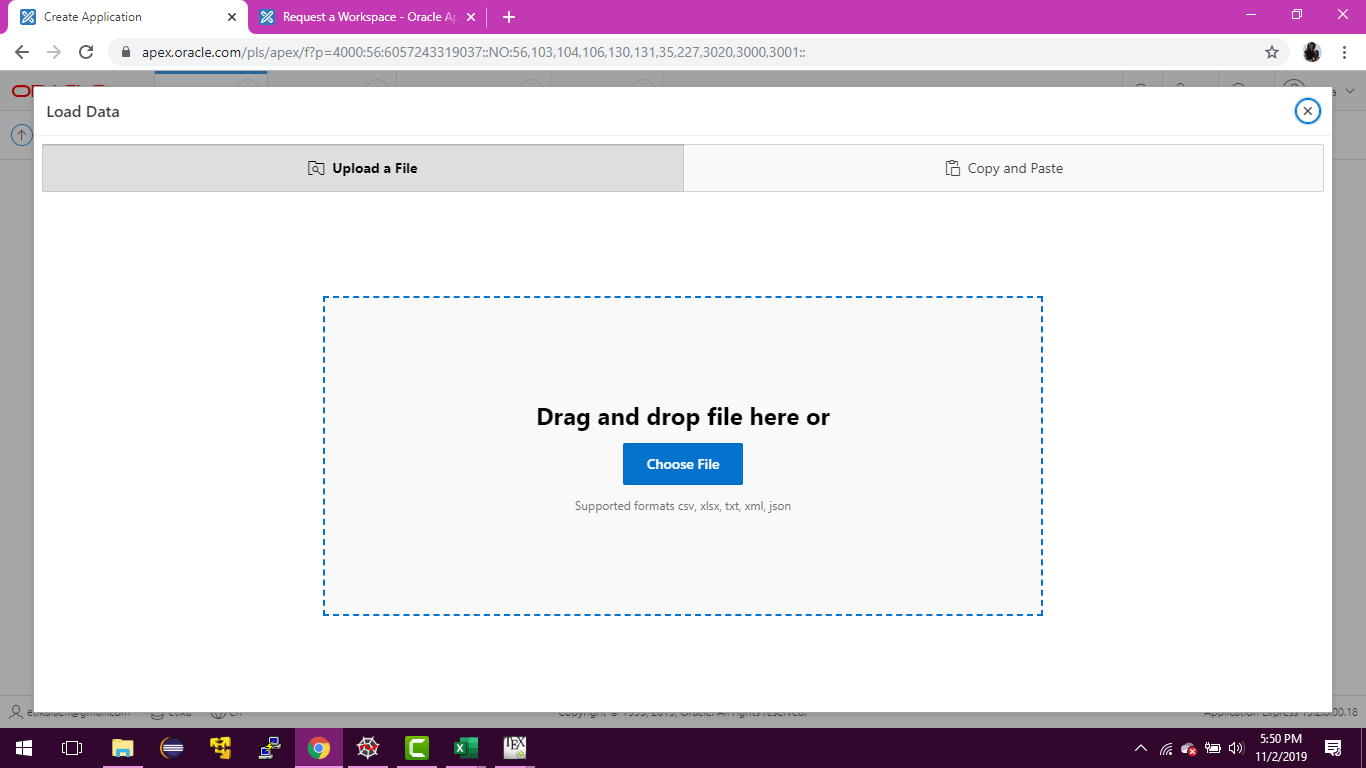
\includegraphics[scale= 0.3]{gambar/7.png}\\
\item drug dan drop file yang akan dijadikan isi dalam tabel\\
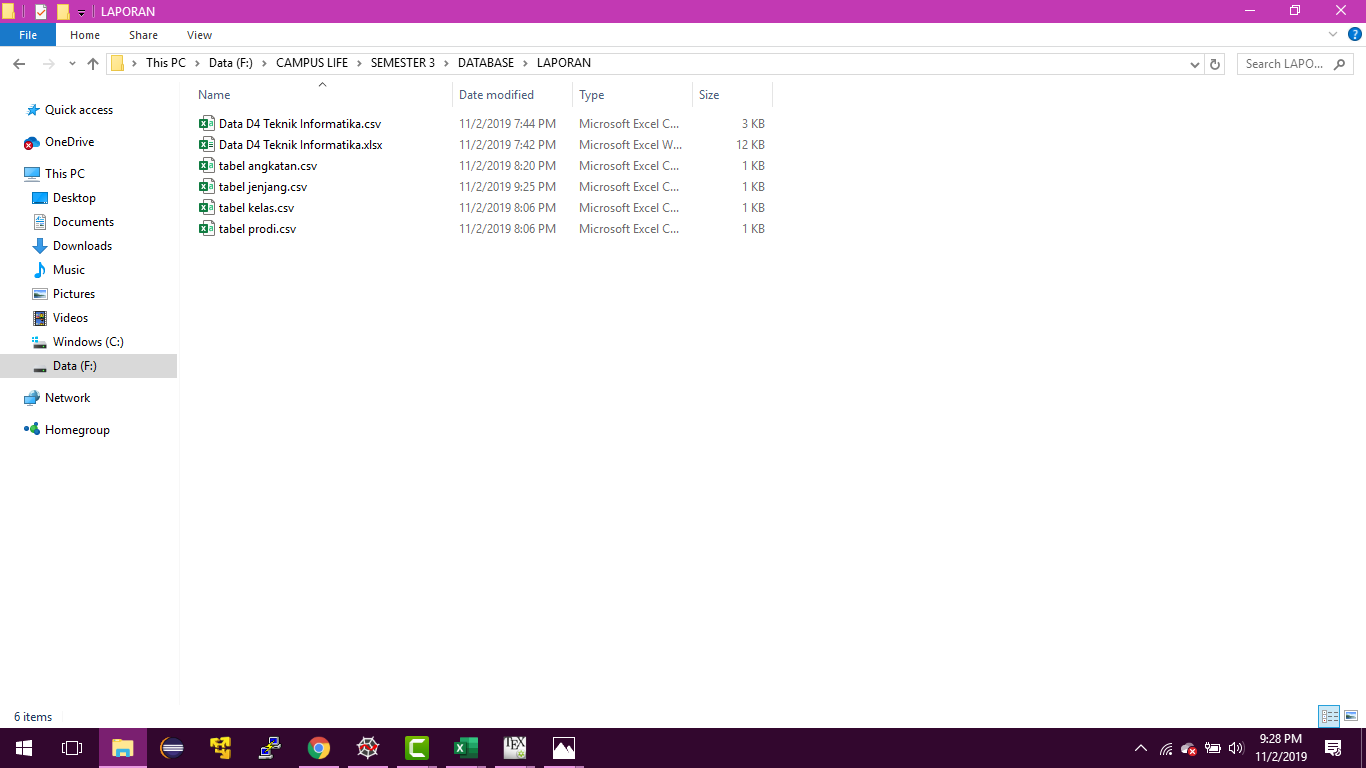
\includegraphics[scale= 0.3]{gambar/8.png}\\
item file yang dimasukan ada beberapa file\\
\item masukan koding danrun satu persatu hingga tidak adakoding yg error\\
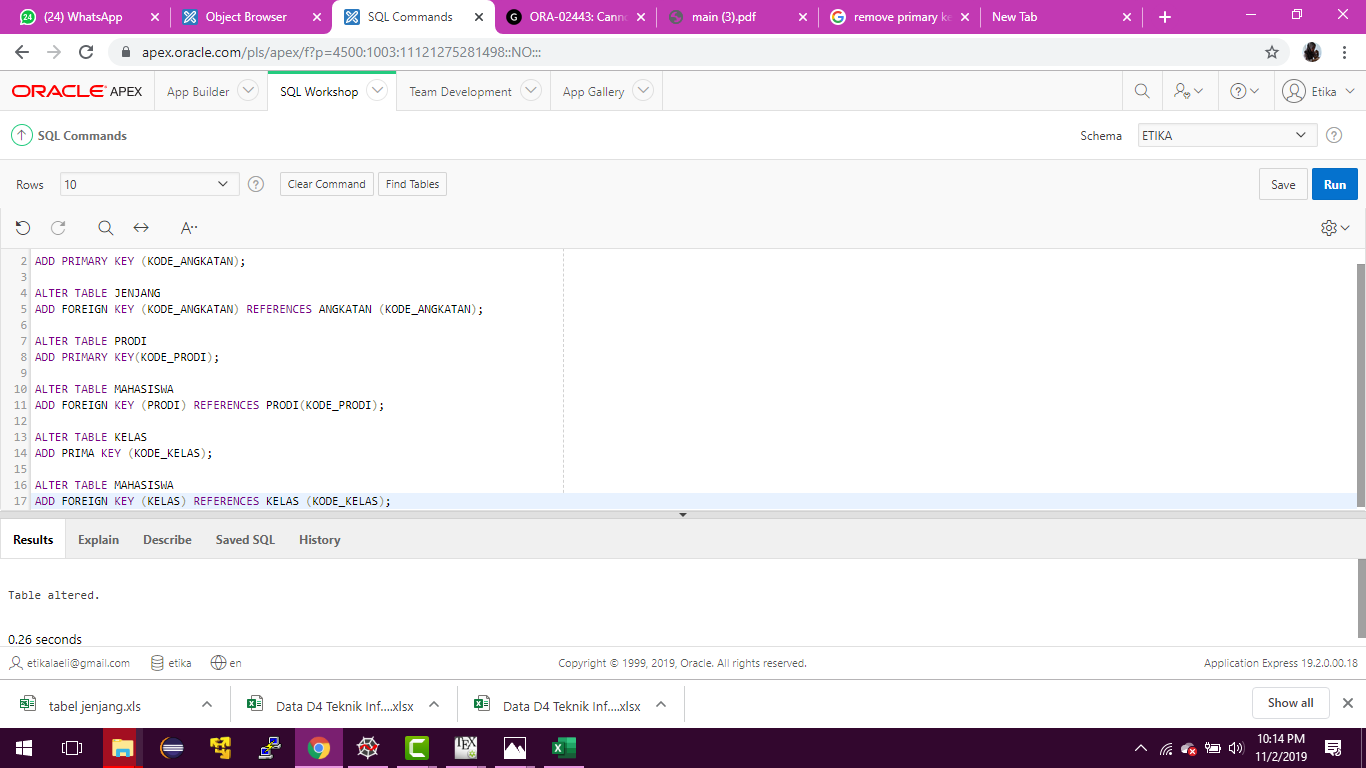
\includegraphics[scale= 0.3]{gambar/9.png}\\
\item lalu kembali ke halaman cretae an application\\
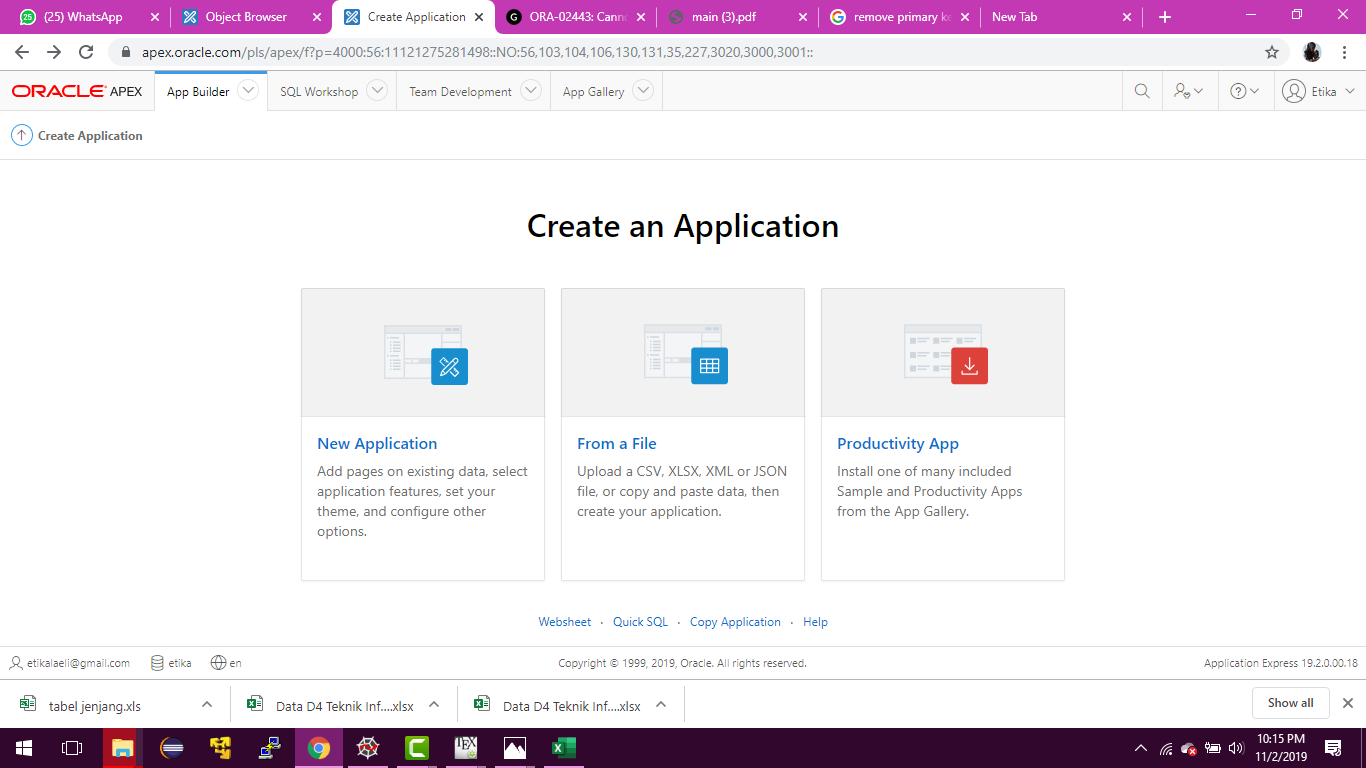
\includegraphics[scale= 0.3]{gambar/10.png}\\
\item buat judul aplikasi\\
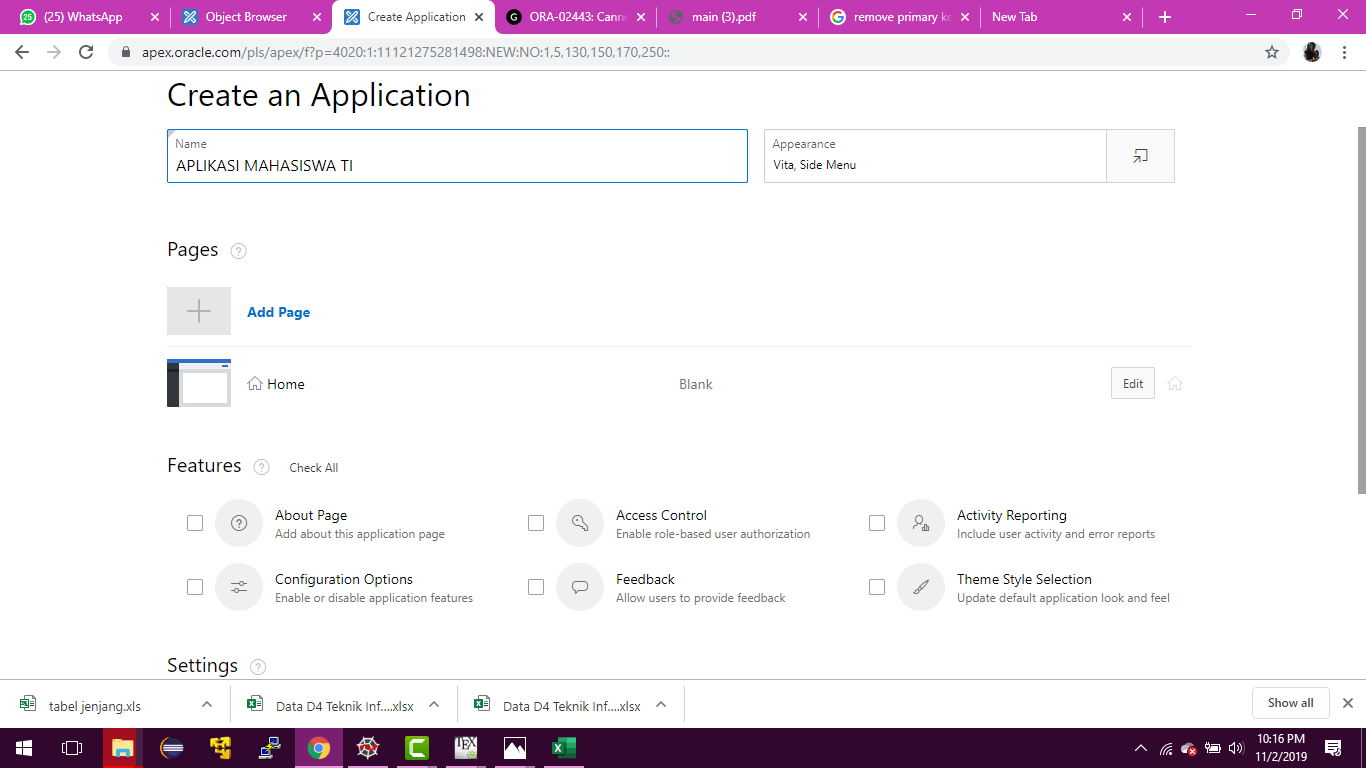
\includegraphics[scale= 0.3]{gambar/11.png}\\
\item klik faceted search\\
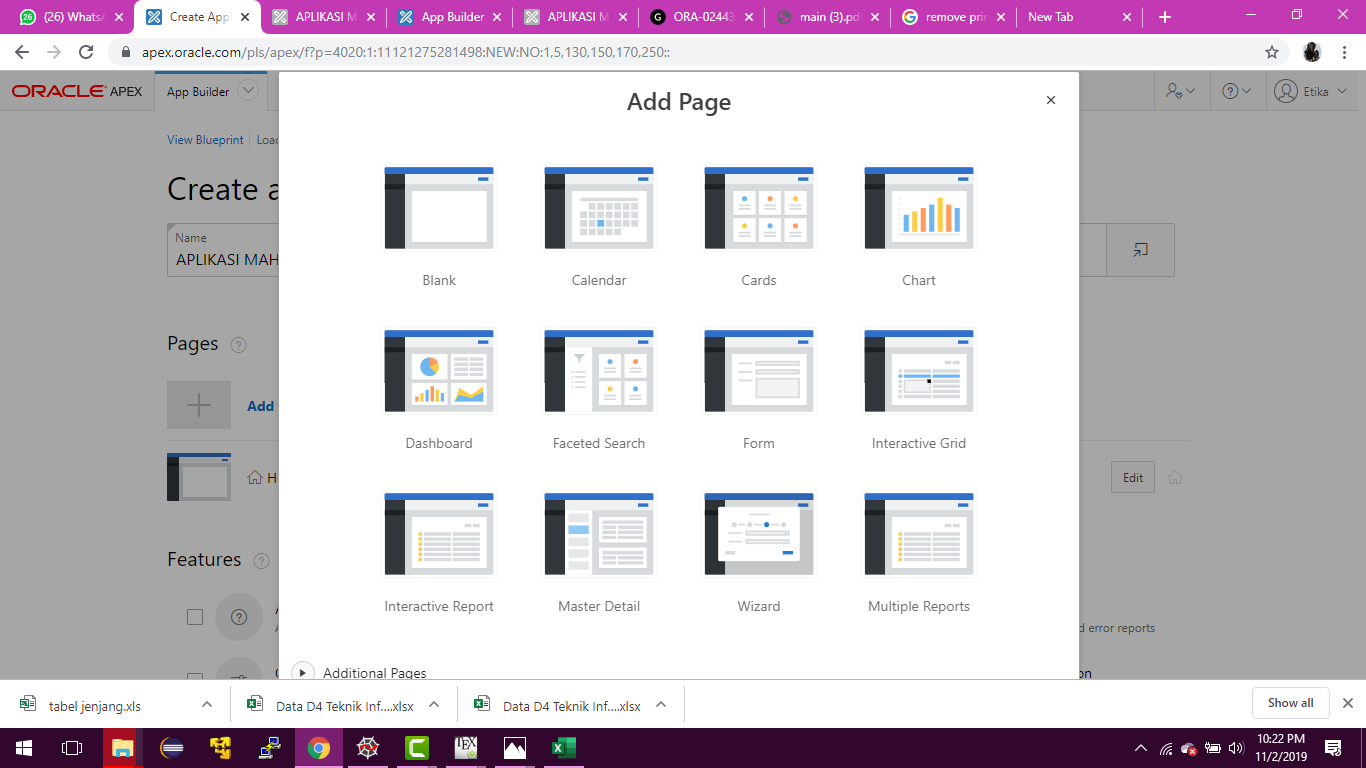
\includegraphics[scale= 0.3]{gambar/12.png}\\
\item pilih table yg akan dijadikan isi dala aplikasi\\
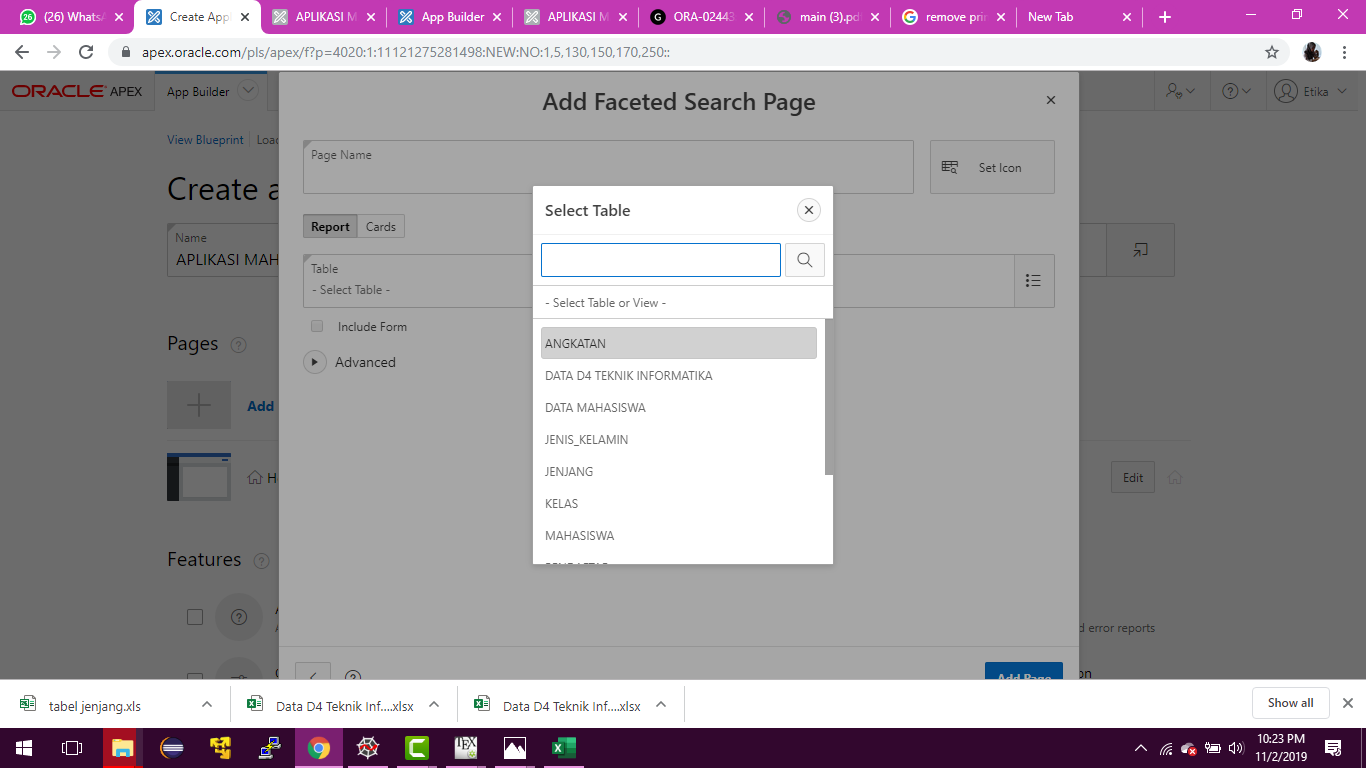
\includegraphics[scale= 0.3]{gambar/13.png}\\
\item sign buat masuk ke dalam aplikasi\\
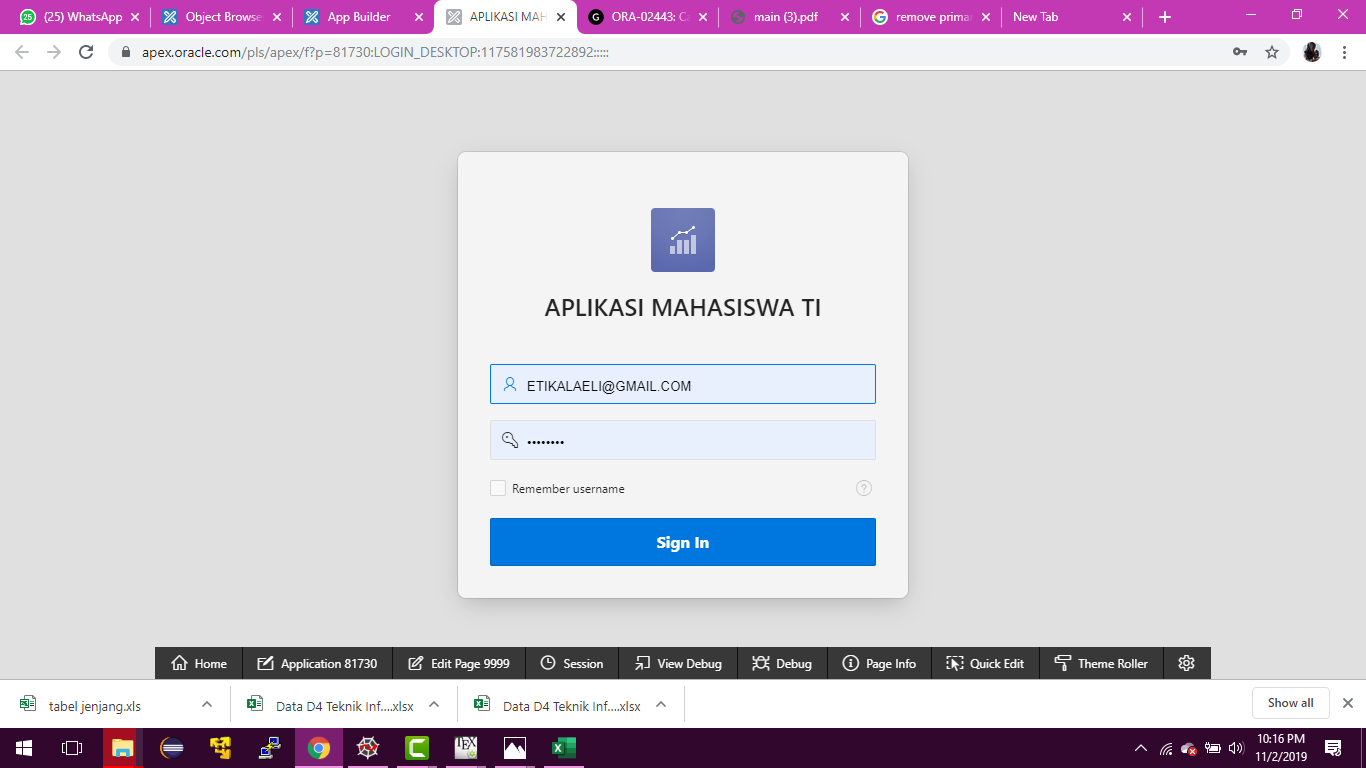
\includegraphics[scale= 0.3]{gambar/14.png}\\

\end{enumerate}

\href{https://apex.oracle.com/pls/apex/f?p=81879:1:19916003679884::NO:::}{LINK APLIKASI}